
\documentclass[10pt,letterpaper]{article}
% Default margins are too wide all the way around. I reset them here
%\setlength{\topmargin}{-.5in} \setlength{\textheight}{9in}
%\setlength{\oddsidemargin}{.125in} \setlength{\textwidth}{6in}

\usepackage{setspace}
\doublespacing

\usepackage{geometry}
\geometry{legalpaper, margin=1in}

\usepackage{pslatex}
\usepackage{apacite}
\usepackage{url}
\usepackage{graphicx}
\usepackage{caption}
\usepackage{subcaption}
\usepackage{listings}
\usepackage{color}
\usepackage{textcomp}
\usepackage{amsmath}
\usepackage{amssymb}
\usepackage{wrapfig}
\usepackage{lipsum}


\graphicspath{{figures/}}

\def\signed #1{{\leavevmode\unskip\nobreak\hfil\penalty50\hskip2em
  \hbox{}\nobreak\hfil(#1)%
  \parfillskip=0pt \finalhyphendemerits=0 \endgraf}}

\newsavebox\mybox
\newenvironment{aquote}[1]
  {\savebox\mybox{#1}\begin{quote}}
  {\signed{\usebox\mybox}\end{quote}}


 \newcommand{\denote}[1]{\mbox{ $[\![ #1 ]\!]$}}

\definecolor{Red}{RGB}{255,0,0}
\newcommand{\red}[1]{\textcolor{Red}{#1}}  

\usepackage{titlesec}

\setcounter{secnumdepth}{4}

\titleformat{\paragraph}
{\normalfont\normalsize\bfseries}{\theparagraph}{1em}{}
\titlespacing*{\paragraph}
{0pt}{3.25ex plus 1ex minus .2ex}{1.5ex plus .2ex}



\title{Generic supplement}


\begin{document}

\maketitle



\appendix


\section{Experiment 1a: \emph{Measuring $P(x)$ for familiar categories}}

The goal of this experiment was to measure participants' beliefs about the distributions of the prevalence of various properties within and across categories.

\subsection{Participants}

We recruited 30 participants over Amazon's crowd-sourcing platform Mechanical Turk (MTurk).  Participants were restricted to those with US IP addresses and with at least a 95\% MTurk work approval rating. All participants were native English speakers. The experiment took about 10 minutes and participants were compensated \$1.00.

\subsection{Procedure and materials}

On each trial of the experiment, the participant filled out a table where each row was an animal category and each column was a property\footnote{The experiment in full can be viewed at \url{http://stanford.edu/~mtessler/experiments/generics/experiments/real-kinds/prior-2.html}}. 
Participants were asked to respond with the percentage of the species that had the property.
The list of animal categories was only partially pre-specified with animal categories that would be used in the generic truth judgment task.
%These names were randomly sampled from a larger set of categories of interest (see Appendix \ref{sec:appendix} for full list of animals and properties used). 
Participants were asked to add five of their own animal names to the list. 
Upon completion, the next column appeared with a property (e.g. ``has manes'') as the column header and text-boxes where the participants could put their estimated prevalence. 
%Participants were asked: ``For each kind of animal, what percentage of the species do you think [property]?'' 
This procedure was repeated for 8 properties in total. 
The animal kind column was unable to be modified once completed. 
The prevalence columns, however, could be modified at a later stage (i.e. the participant could go back and change her estimates after seeing more properties). 
Participants completed this procedure on each of 2 trials.

We used a set of properties associated with generics of theoretical interest (16 properties in total), motivated in part by conceptual distinctions pointed out by \citeA{Prasada2013}. 
The conceptual categories used to generate the generics were: majority characteristic (e.g. ``Leopards have spots''), minority characteristic (e.g. ``Lions have manes''), striking (e.g. ``Sharks attack swimmers.''), and majority false generalizations (e.g. ``Ducks are female.'') \cite{Prasada2013}. In addition, we included false sentences (e..g ``Lions lay eggs''), to cover the full range of possible truth values .
For a full list of the generic sentences used in this experiment, see Appendix \ref{sec:appendix}.
Complete instructions given to participants can be seen in Appendix \ref{sec:prior1instruct}.



\subsection{Bayesian data analysis}
\label{sec:bda1}

There is important latent structure in the prior elicitation task. We will describe the model from the perspective of inferring the distribution of a particular property (e.g. ``lays eggs''). 
The same general structure is implemented for each item independently, with the slight except that the item-wise models share a data-analytic noise parameter $\phi$, described in more detail below. 

Responses $d$ can be categorized into those that reflect the property is either present or absent in the species. 
If the property is absent, then the response is 0\% (of the species has the property). 
The number of 0 responses act as an indicator of the prevalence of the property \emph{across categories} $\theta_{across}$ (for example, ``are female'' would have very few 0\% responses, whereas ``lays eggs'' would receive appreciably more, owing to the fact the prevalence of these properties \emph{across categories} is different). \emph{A priori}, we assume nothing about the prevalence across categories $\theta_{across} \sim \text{Uniform} (0, 1)$. 
%
\begin{align*}
d_{across} & \sim \text{Bernoulli}(\theta_{across}) \\
d_{across} & = \begin{cases}
				1 & \mbox{if } d > 0 \\
				0 & \mbox{if } d = 0 
				\end{cases}
\end{align*}
%
For those responses that reflect the property is present ($d > 0$), we assume those responses come from a distribution with unknown mean ($\gamma_{within}$) and variance ($\delta_{within}$). 
Since the responses vary between 0 - 100, the natural distribution is a Beta distribution. 
We model the observed data as being generated by a mixture of this model and a model of random guessing behavior. 
Modeling random guessing explicitly is important for recovering reliable estimates of the parameters of the model, which would otherwise be contaminated by this data \cite{LW2014}. 
%
\begin{align*}
d_{within} \sim \begin{cases}
					\text{Beta}(\gamma_{within}, \delta_{within})  &  \mbox{ if } d_{observed} > 0 \text{ and }  \text{Bernoulli} (\phi) = 0 \\
					\text{Uniform}(0,1) & \mbox{ if } \text{Bernoulli} (\phi) = 1
				\end{cases}
\end{align*}
%
In principle, $\phi$ could be vary by participant (some participants produce noisier data than others). For simplicity, we assume some global ``guessing rate'', and thus $\phi$ is an experiment-wide variable.
We make no assumptions about the amount of noise in the data and we put uninformative priors over it, as well as over the means and concentrations of the prevalence distributions. 
%
\begin{align*}
 \phi \sim \text{Uniform}(0,1) \\
\gamma_{within} \sim \text{Uniform}(0,1) \\
\delta_{within} \sim \text{Uniform}(0,50)
\end{align*}
%
We implemented this Bayesian statistical model using the probabilisitic programming language WebPPL \cite{dippl}. We used the Metropolis-Hastings algorithm to estimate the posterior distribution over the latent parameters $\theta_{across}, \gamma_{within}, \delta_{within}, and \phi$ with X chains of Y samples.

To reconstruct the likely distribution of  prevalence reflecting both within- and across- category prevalence, we took samples from the posterior predictive distribution of $d$ by running the forward model: 
%
\begin{align*}
h & \sim \text{Bernoulli}(\theta_{across}) \\
x & \sim \begin{cases} 
		\text{Beta}(\gamma_{within}, \delta_{within}) &\mbox{if } h = 1 \\ 
				0 & \mbox{if } h=0
				\end{cases} 
\end{align*}
%
where, $h$ is a variable indicating whether or not the property is present within a particular species. 

We also estimated the likely prevalence of each animal category and property pair of interest (e.g. the prevalence of ``laying eggs'' among ``Ducks''), to be used as the measure of prevalence in the generic truth judgment task (Expt.~1b). 
For this, we assume the data was generated from a Beta distribution with unknown mean and concentration. 
We also assume some global amount of noise in the data.

\begin{align*}
d \sim \begin{cases}
					\text{Beta}(\gamma, \delta)  &  \mbox{ if } \text{Bernoulli} (\phi) = 0 \\
					\text{Uniform}(0,1) & \mbox{ if } \text{Bernoulli} (\phi) = 1
				\end{cases}
\end{align*}




\section{Experiment 1b: \emph{Truth judgments of natural cases}}

The goal of this experiment was to measure participants' beliefs about the acceptability of a number of different generic sentences. 

\subsection{Participants}

We recruited 100 participants over Amazon's crowd-sourcing platform Mechanical Turk (MTurk).  Participants were restricted to those with US IP addresses and with at least a 95\% MTurk work approval rating. All participants were native English speakers. The experiment took about 3 minutes and participants were compensated \$0.35.

\subsection{Procedure and materials}

We used a two-alternative forced-choice (2AFC) paradigm to measure participants' beliefs about the acceptability of 30 generic sentences. 
Data reported in \citeA{Prasada2013} revealed that participants assign midpoint ratings on a Likert scale to anomalous generics like ``Birds are female''. 
We hypothesized that these ``neither true nor false'' ratings would be translated into more graded responses across the population using the 2AFC (i.e. subjects would be closer to chance).

Participants were asked to report whether they agreed or disagreed with generic sentences presented in bare plural form (e.g. ``Birds lay eggs.''). 
Items were presented sequentially, and participants reported whether or not they agreed with the sentence by pressing either ``P'' or ``Q'' (randomized between-subjects). 

Generic sentences were selected to correspond with the prevalence distributions elicited in Expt.~1a. 
They covered a range of conceptual categories: Characteristic (e.g. ``Ducks have wings.''), Minority (e.g. ``Lions have manes.''), Striking (e.g. ``Mosquitos carry malaria.''), False generalization (e.g. ``Lions are male.''), and false (e.g. ``Lions lay eggs.'').
Approximately 10 true, 10 false, and 10 uncertain truth-value generics were selected (see Appendix \ref{sec:appendix} for full list of items).
As a manipulation check, participants were asked at the end of the trials which button corresponded to ``Agree''.

\subsubsection{Results}

Four participants were excluded for failing to successfully report which button corresponded with ``Agree''. 
Five additional participants were excluded for listing a language other than English as their native language, resulting in 91 participants.


\begin{figure}
\centering
    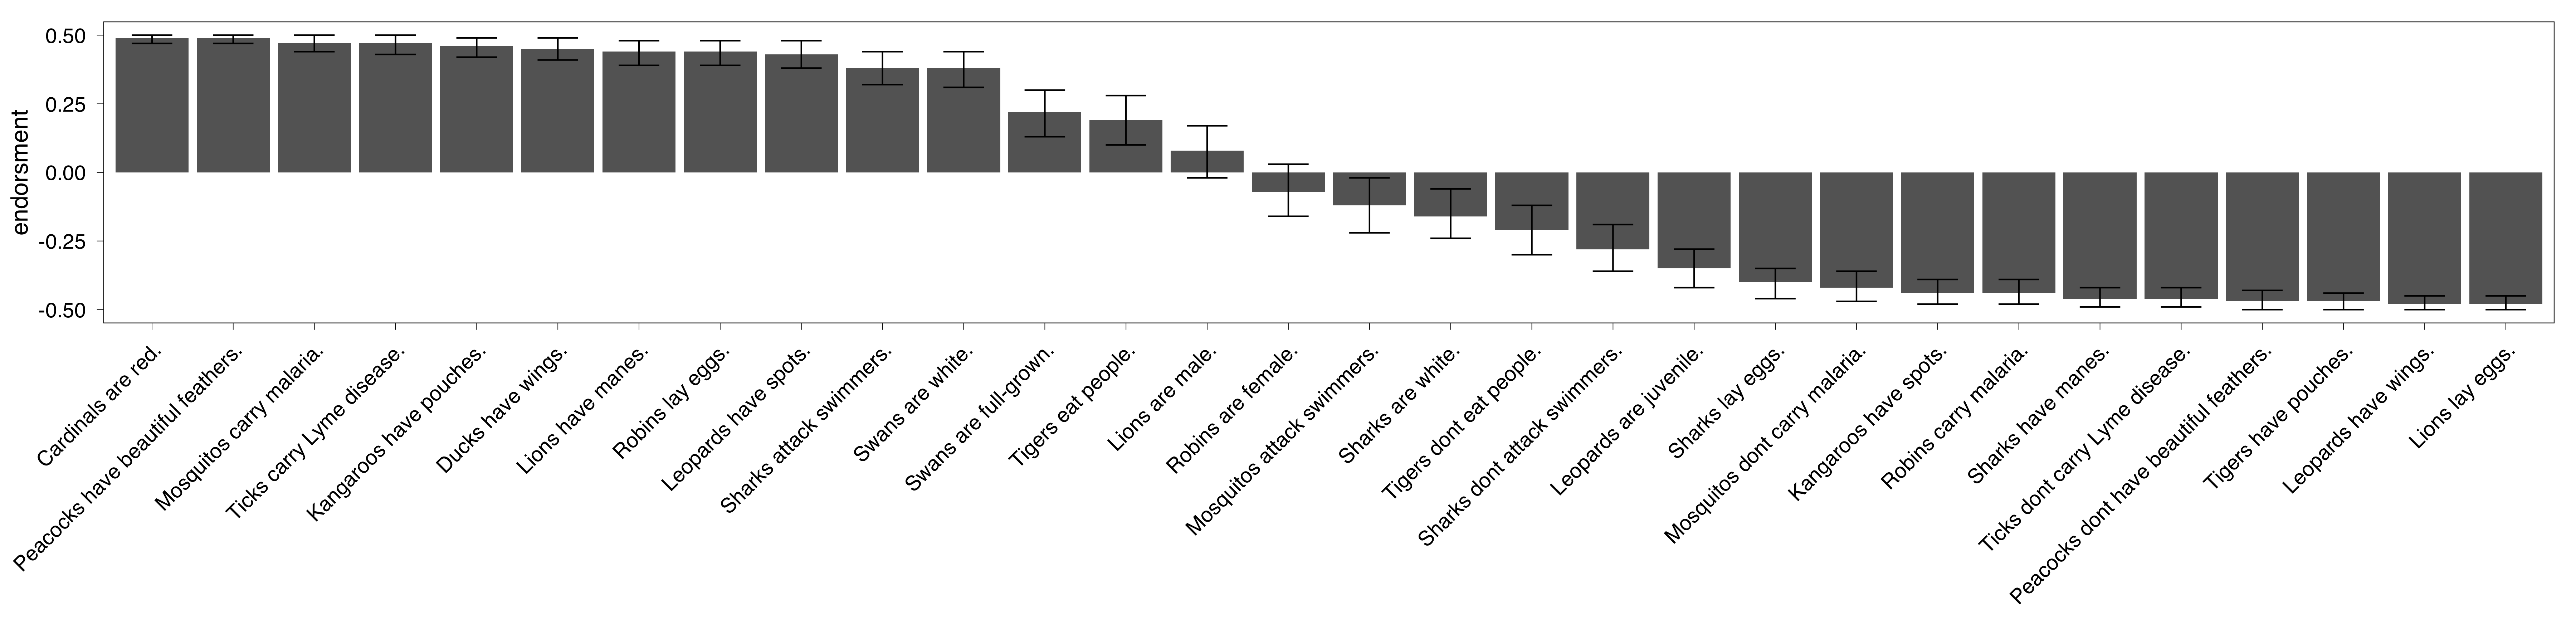
\includegraphics[width=\columnwidth]{truhtjudge_n100}
    \caption{Truth judgments from Expt.~1b for each item. Y-axis denotes deviations from chance in the 2AFC. There is large agreement for both generics which are true and generics which are false. There is considerable disagreement across participants for a number of ``neither true nor false'' generic statements. }
  \label{fig:tj1b}
\end{figure}


The 30 generic sentences fell into 3 \emph{a priori} categories: definitely true, definitely false, and neither true nor false (Figure \ref{fig:tj1b}). 
We entered participants' agreement judgments into a mixed-effect logistic regression with random by-participant effects of intercept. 
This \emph{a priori} distinction was a significant predictor of the eventual truth judgments: true generics were significantly more likely to be agreed with than the indeterminate generics ($\beta = 3.14; SE = 0.15; z = -20.9$).
Indeterminate generics were agreed with \emph{less} likely than chance ($\beta = -0.49; SE = 0.09; z = -5.3$) but significantly more than false generics ($\beta = 2.07; SE = 0.15; z = 14.1$).

Truth judgments for these generic sentences were correlated with the prevalence of the property for the target category elicited in Expt.~1a ($r = 0.73$, Figure \ref{fig:scatterprev}). This is, of course, expected given that high-prevalence true generics (e.g. ``Leopards have spots.'') and low-prevalence false generics (e.g. ``Leopards have wings.'') were used. 
However, large deviations from a purely within-category prevalence account remain: Generics with intermediate prevalences (Prevalence quartiles 2 and 3: $ 22\% < prevalence < 62\%$), exhibited no correlation with truth judgments ($r_{Q2,3} = -0.08$).


\begin{figure}
\centering
    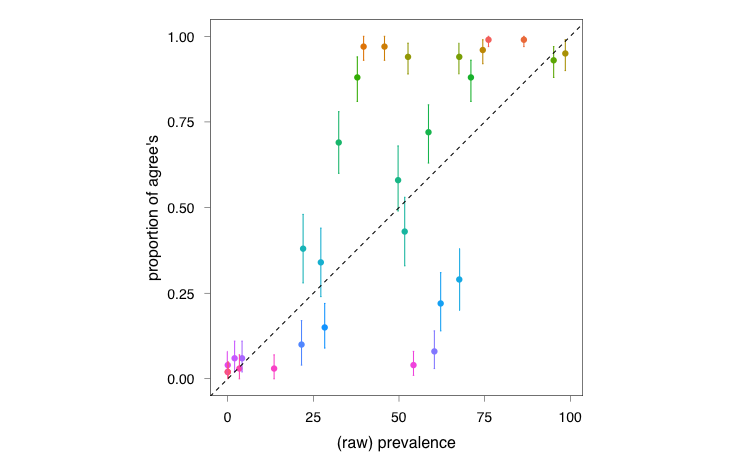
\includegraphics[width=0.8\columnwidth]{tj_n50_tjVsPrevalence}
    \caption{Truth judgments from Expt.~1b for each item vs. the prevalence of the property for the target item as measured in Expt.~1a. For example, ``Leopards have spots'' has a very high truth judgment (Expt.~1b; Y-axis), and ``has spots'' is a highly prevalent property for leopards (Expt.~1a; X-axis). Color spectrum corresponds to the rank ordering of the truth judgment data; similarly colored dots received similar truth judgments.}
  \label{fig:scatterprev}
\end{figure}




\subsection{Lifted-threshold model predictions}

The speaker model specified in Section \ref{sec:model} reasons about the likely prevalence that a listener will infer given  a generic sentence and assuming an informative speaker and a distribution over the prevalence of the property. 
In this way, the model takes into account the prevalence of the property both within- and across-categories as well as communicative principles.
We explore the predictions of this model, using the empirical priors elicited in Expt.~1a. 
We compare these predictions to the truth judgment data observed in Expt.~1b.

\subsubsection{Posterior over model parameters}

The full model has one free parameter, the speaker rationality $\lambda$ in Equation \ref{eq:S1}, and one data analytic parameter, a contamination parameter $\phi$.
To learn about the \emph{a posteriori} credible values of our model parameters, we used the probabilistic programming language WebPPL \cite{dippl} to collect \red{X} chains of \red{Y} samples using the Metropolis-Hastings algorithm. 
The speaker rationality parameter represents the speaker's belief in how rational the hypothetical listener believes he is when choosing to say the generic (over saying nothing). 
The 95\% Highest Probability Density (HPD) Interval is [7.86,10.29].

In the data analysis, we also include a contamination parameter $\phi$ to account for noise in the data.  
This represents the proportion of the data that can be better explained by random guessing than by our model of generic language.
In this way, $\phi$ provides a crude measure of goodness of fit. 
The 95\% HPD Interval is [0.006,0.05]. 
This suggests that there is not a substantial amount of noise in the data, possibly owing to the simplicity of the task. 


\subsubsection{Posterior predictive}

We evaluate the model by examining the posterior predictive distribution of responses. The posterior predictive distribution marginalizes over the inferred parameter values to produce predictions about what the data should look like given the lifted-threshold model and the observed data. This is akin to fitting the parameters and is an important step in model validation: It shows what data is actually predicted by the model. 
Figure \ref{fig:modeldataScatter} shows the Maximum A-Posteriori (MAP) values of the model predictions compared against the observed data. 
The model predicts graded endorsements for the generic statements used in Expt.~1b. 



\subsection{Discussion}

In Expt.~1, we asked whether or not participants' truth judgments on a set of generic sentences covering a range of conceptual distinctions could be explained by a language understanding model with a truth-functional threshold sensitive to the prior distribution over prevalence. 
In Expt.~1a, we empirically measured the prior distribution of prevalence by asking participants about the prevalence of certain properties across many animal categories. 
Here, we observed qualitatively different distributions corresponding to properties that are common within-categories and common across-categories (e.g. ``are male''), common within-categories but rare across-categories (e.g. ``have manes''), rare within-categories and rare across-categories (e.g. ``carries malaria''). Interestingly, these same distinctions are made between generics of these properties \cite{Prasada2013}. 
Our empirical and modeling results suggest these distinctions are a result of different belief distributions about the prevalence of the properties.

How does the model arrive at different truth judgments for generics of different properites?
Here, the prevalence prior plays a critical role in determining where the generic-threshold $\theta$ (and, consequently, the resulting inferred prevalence $x$) is likely to fall (see Figure \ref{fig:priors1a} for examples of the relevant priors). 
In setting the threshold, the pragmatic listener $L_{1}$ balances the truth of the utterance with the informativeness of the utterance. 
If the pragmatic listener hears ``Lions haves manes.'', she will likely set the threshold $\theta$ below 50\%, as this is necessary to make the utterance true (Figure \ref{fig:priors1a} bottom left). 
At the same time, the listener believes the message to be informative, so she will probably set $\theta$ above 10\%. 
Since the posterior inferred prevalence has to be greater than the threshold in order to make the utterance true, the expected value of inferred prevalence $x$ will be about 50\% (i.e. after ruling out everything below 10\% and integrating over the conditional distribution, the inference is that 50\% of the species has the property). 
Since this matches the speaker's known prevalence of having manes among lions, the speaker concludes the generic is a helpful thing to say (relative to saying nothing, or saying the opposite).
At the same time, participants judged ``Lions are male'' to be neither true nor false; the model exhibits the same behavior because the prevalence of being male among lions is neither significantly more nor less than prevalence of being male among other animal species. 
Our model of a speaker considering a listener who has uncertainty about the true threshold on prevalence produces truth judgments highly similar to those of our participants.





\section{Stimuli used in Experiment 1}
\label{sec:appendix}	

\begin{table}[h]
\begin{tabular}{| l || l | l | l |}
\hline
Conceptual type               & Item                    & Truth judgment & Prevalence estimate \\
\hline \hline
Majority characteristic       & 1. Leopards have spots.    &                &                     \\
                                          & 2. Ducks have wings.                       &                &                     \\
                                          & 3. Cardinals are red.                       &                &                     \\
                                          & 4. Swans are white.                       &                &                     \\
Minority characteristic       & 5. Lions have manes.       &                &                     \\
                                          & 6. Kangaroos have pouches.                        &                &                     \\
                                          & 7. Robins lay eggs.                        &                &                     \\
Striking                      & 8. Sharks attack swimmers. &                &                     \\
                                  & 9. Mosquitos carry malaria.                        &                &                     \\
                                  & 10. Ticks carry lyme disease.                        &                &                     \\
                                  & 11. Tigers eat people.                        &                &                     \\
Majority false generalization & 12. Robins are female.      &                &                     \\
                                              & 13.  Lions are male.                       &                &                     \\
False                         & 14. Leopards have wings.       &                &                    \\
                                              & 15. Kangaroos have spots.                       &                &                     \\
                                              & 16.  Tigers have pouches.                       &                &                     \\
                                              & 17.  Robins carry malaria.                       &                &                     \\
                                              & 18. Sharks have manes.                       &                &                     \\
                                              & 19. Lions lay eggs.                       &                &                     \\
                                              & 20. Swans attack swimmers.                       &                &                     \\
Novel                         & 21. Mosquitos attack swimmers.       &                &                    \\
                         & 22. Sharks lay eggs.       &                &                    \\
                         & 23. Frogs have spots.       &                &                   \\
\hline

\end{tabular}
\caption{Stimuli used in Experiment 1.}
\label{tab:expt1}
\end{table}


\section{Instructions used in Experiment 1a: prior elicitation for familiar categories}
\label{sec:prior1instruct}

Participants were told 
\begin{quote}
In this study, we are interested in how prevalent certain properties are within different kinds of animals. We will give you examples of the kinds of animals we have in mind and ask you to list a few of your own.

Then, you will estimate the \emph{percentage of the individual members} of the animal species that have certain properties.

On each trial, you will rate 8 properties. The properties will be revealed to you one at a time. Essentially, you will be filling out a big table. You are allowed to go back and revise your answers, if you think there is a more realistic estimate you could give. You will do this 2 times (2 big tables). 

\end{quote}


\section{Instructions used in Experiment 2a: prior elicitation for novel categories}
\label{sec:prior2instruct}

Participants were again told they were on a newly discovered island with lots of new animals on it. They were then given the following instructions

\begin{quote}
One day, you are roaming through the library when you encounter a data-collection robot. The robot doesn't know very much about the world and is asking you questions to learn more. Today, it wants to learn about properties of animals. It is randomly selecting an animal from its memory and a property from its memory, and asking you if the animal is likely to have the property.

Of course, you're new to this island so you don't really know anything about these animals. The properties, however, will be familiar. Try to provide your best guess given your own experience.
\end{quote}

Participants were then run through a practice trial where they were familiarized with the questions that would be asked on them. 
On each trial, the data-collection robot introduced a new animal (e.g. ``We recently discovered animals called glippets.''). 
The robot then asked how likely it was that ``there was \emph{a} glippet with [[property]]''. 
This question aimed to get at the prevalence of the property \emph{across} categories (e.g. it's very likely that there is a glippet that is female, less likely that there is a glippet that has wings, and even less likely that there is a glippet has purple wings). 
The second question was about the prevalence \emph{within} categories. The robot asked, ``Suppose there is a glippet that has wings. What percentage of glippets do you think have wings?''

\section{Stimuli used in Experiment 2}
\label{sec:materials2}

Many of these materials were originally used in \citeA{Cimpian2010}.

\begin{table}[h]
\begin{tabular}{| l || l | l | l |}
\hline
Property type               & Item                    & Across-category prevalence estimate  & Within-category prevalence estimate \\
\hline \hline
Body part       			& 1. Teeth    &   &                     \\
                                          & 2. Fur                       &                &                     \\
                                          & 3. Tails                     &                &                     \\
                                          & 4. Claws                       &                &                     \\
                                          & 5. Feathers                       &                &                     \\
                                          & 6. Ears                       &                &                     \\
                                          & 7. Legs                       &                &                     \\
                                          & 8. Skin                       &                &                     \\
Colored part      	 & 9. Pink teeth       &                &                     \\
                                          & 10. Yellow fur                       &                &                     \\
                                          & 11. Orange tails                         &                &                     \\
                                          & 12. Blue claws                       &                &                     \\
                                          & 13. Purple feathers                      &                &                     \\
                                          & 14. Orange ears                    &                &                     \\
                                          & 15. Silver legs                       &                &                     \\
                                          & 16. Violet skin                      &                &                     \\       
Vague part      	 & 17. Long teeth       &                &                     \\
                                          & 18. Curly fur                       &                &                     \\
                                          & 19. Long tails                         &                &                     \\
                                          & 20. Big claws                       &                &                     \\
                                          & 21. Smooth feathers                      &                &                     \\
                                          & 22. Small ears                    &                &                     \\
                                          & 23. Long legs                       &                &                     \\
                                          & 24. Rough skin                      &                &                     \\ 
Common accidental part    & 25. Wet fur       &                &                     \\
                                          & 26. Dusty skin                       &                &                     \\
                                          & 27. Worn-out claws                         &                &                     \\
                                          & 28. Fungus-covered fur                      &                &                     \\
                                          & 29. Muddy feathers                      &                &                     \\
                                          & 30. Rotten teeth                   &                &                     \\
                                          & 31. Torn feathers                       &                &                     \\
                                          & 32. Itchy tails                      &                &                     \\  
Rare accidental part    & 33. Sore legs       &                &                     \\
                                          & 34. Torn tails                       &                &                     \\
                                          & 35. Cracked claws                         &                &                     \\
                                          & 36. Sore teeth                       &                &                     \\
                                          & 37. Swollen ears                      &                &                     \\
                                          & 38. Infected ears                    &                &                     \\
                                          & 39. Burned skin                       &                &                     \\
                                          & 40. Broken legs                     &                &                     \\                                                                                          
                                           \hline

\end{tabular}
\end{table}

\bibliographystyle{apacite}

\setlength{\bibleftmargin}{.125in}
\setlength{\bibindent}{-\bibleftmargin}

\bibliography{generics}

\end{document}

